%!TeX root=../main.tex

% -- * What we talk about when we talk about search * --
\textbf{Topology Search}\: 
The operators used to search for neural network topologies are inspired by the well-established neuroevolution algorithm NEAT~\cite{neat}. 
%
While in NEAT the topology and weight values are optimized simultaneously, we ignore the weights and apply only topological search operators.
%

The initial population is composed of sparsely connected networks, networks with no hidden nodes and only a fraction of the possible connections between input and output. 
%
New networks are created by modifying existing networks using one of three operators: insert node, add connection, or change activation (Figure \ref{fig:topsearch}). 
%
To insert a node, we split an existing connection into two connections that pass through this new hidden node.
%
The activation function of this new node is randomly assigned. 
%
New connections are added between previously unconnected nodes, respecting the feed-forward property of the network. 
%
When activation functions of hidden nodes are changed, they are assigned at random.
%
Activation functions include both the common (e.g. linear, sigmoid, ReLU) and more exotic (Gaussian, sinusoid, step), encoding a variety of relationships between inputs and outputs. 

%!TeX root=../main.tex

% TODO: 
%   - Update activation pic


\begin{figure}[h!]        
\vskip -0.05in % useful knobs to optimize layout
    \centering        
    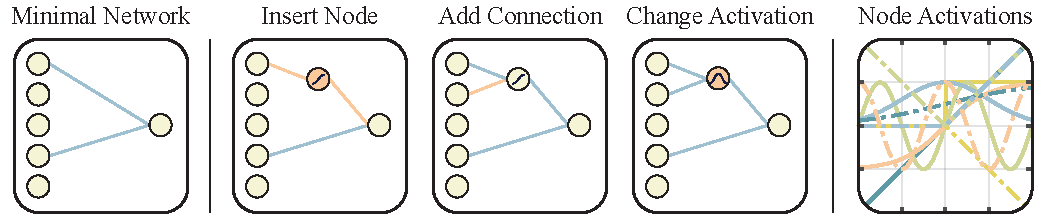
\includegraphics[width=1\textwidth]{img/topOper.pdf}  
\vskip -0.05in % useful knobs to optimize layout
    \caption      
    {     
        \textit{Operators for Searching the Space of Network Topologies}
        \newline
        \textit{Left:} A minimal network topology, with input and outputs only partially connected. 
        \newline
        \textit{Middle:} Networks are altered in one of three ways. \textit{Insert Node}: a new node is inserted by splitting an existing connection. \textit{Add Connection}: a new connection is added by connecting two previously unconnected nodes. \textit{Change Activation}: the activation function of a hidden node is reassigned.
        \newline % DH: added for readabiliy
        \textit{Right:} Possible activation functions (linear, step, sin, cosine, Gaussian, tanh, sigmoid, absolute value, invert (i.e. negative linear), ReLU) shown over the range $[2,2]$.
        }         
    \label{fig:topsearch}   
\vskip -0.05in % useful knobs to optimize layout
\end{figure}


% -- * How and why we rank by complexity * --
\textbf{Performance and Complexity}\: 
% Evaluation
Network topologies are evaluated using several shared weight values. 
%
At each rollout a new weight value is assigned to \textit{all} connections, and the network is tested on the task. 
%
In these experiments we used a fixed series of weight values ($[-2,-1,-0.5,+0.5,+1,+2]$) to decrease the variance between evaluations.\footnote{Variations on these particular values had little effect, though weight values in the range $[-2,2]$ showed the most variance in performance. Networks whose weight values were set to greater than 3 tended to perform similarly -- presumably saturating many of the activation functions. 
%
Weight values near 0 were also omitted to reduce computation, as regardless of the topology little to no information is passed to the output.}
%
We calculate the mean performance of a network topology by averaging its cumulative reward over all rollouts using these different weight values.
%

%
Motivated by algorithmic information theory~\cite{solomonoff1964formal}, we are not interested in searching merely for \textit{any} weight agnostic neural networks, but networks that can be described with a minimal description length~\cite{rissanen1978modeling,grunwald2007minimum,rissanen2007information}. 
%
Given two different networks with similar performance we prefer the simpler network. 
%
By formulating the search as a multi-objective optimization problem~\cite{konak2006multi,mouret2011novelty} we take into account the size of the network as well as its performance when ranking it in the population.

We apply the connection cost technique from \cite{clune2013evolutionary} shown to produce networks that are more simple, modular, and evolvable.
%
Networks topologies are judged based on three criteria: mean performance over all weight values, max performance of the single best weight value, and the number of connections in the network. 
%
Rather than attempting to balance these criteria with a hand-crafted reward function for each new task, we rank the solutions based on dominance relations~\cite{nsga2}.
%
% using the fast non-dominated sorting algorithm introduced as part of the NSGA-II algorithm~\cite{nsga2}, a widely-used standard for multi-objective optimization. 


%When networks are ranked in this way any growth in complexity must be accompanied by an improvement in performance in order for the network to raise in rank. 
Ranking networks in this way requires that any increase in complexity is accompanied by an increase in performance.
%
While encouraging minimal and modular networks, this constraint can make larger structural changes -- which may require several additions before paying off -- difficult to achieve. 
%
%When multiple structures must be added to yield an increase in performance, strict enforcement of this constraint can prevent the necessary stepping stones from ever being laid. 
%
To relax this constraint we rank by complexity only probabilistically: in 80\% of cases networks are ranked according to mean performance and the number of connections, in the other 20\% ranking is done by mean performance and max performance.



%\textbf{Weight Agnostic Neural Network Search}\:%
% Reintroduce goals and approach (unnecessary?)
% Weight Agnostic Neural Networks illustrate that the skills and knowledge required to effectively perform tasks can be encoded entirely within the architecture of a neural network. 
%By substituting weight training with sampling of a single shared weight the space of architectures can be searched without searching the space of weights. Searching for networks with low complexity and high performance allows us to find simple networks which perform well with a variety of weight values.
%
% Weight training is substituted with sampling of a single shared weight value for all weights, allowing us to search the space of architectures without searching the space of weights. By searching for networks with both low complexity and high performance we find simple networks that perform well with a variety of weight values. 
%
% - Detailed Procedure - 
% Initialization
% We begin with an initial population of sparsely connected neural networks. These networks contain no hidden nodes, and each input is connected to each output only with some slight probability. As the search progresses more nodes and connections are added, but by beginning with a population of minimal networks the most important input/output connections are quickly identified. 

% % Evaluation
% Each network in the population is evaluated using several weight values. At each rollout a new weight value is assigned to \textit{all} connections, and the network is tested on the task. This weight value is drawn from a uniform zero mean distribution; though in these experiments a fixed series is used ($[-2,-1,-0.5,+0.5,+1,+2]$) to decrease the variance between evaluations\footnote{Variations on these particular values had little effect, though weight values between -2 and 2 showed the most variance in performance. Networks whose weight values were set to greater than 3 tended to perform similarly -- presumably saturating many of the activation functions. Weight values near 0 were also omitted, as regardless of the topology nearly no signal is sent to the output}. The performance of a network is calculated based on the reward earned over all trials.
% The population of networks is then ranked by performance and complexity. 

% % Selection and Variation
% A new population is then created. The very highest ranking networks are copied to the new population without alteration, and the remainder of population is filled with variations of the best networks. Parent networks are chosen probabilistically using tournament selection~\cite{tournamentSelection}: a number of networks are chosen at random, and the highest ranked of the group is chosen as a parent. This parent is varied by adding nodes, connections, or changing the activation function of one of the hidden nodes, and added to the new population. The new population is then evaluated, ranked, and the process repeats.